\chapter{Cargador MPPT}
    
        \section{¿Qué es MPPT?}
        
            \textit{Maximum Power Point Tracking} es una técnica utilizada en cargadores para obtener la máxima potencia posible cuando las condiciones de alimentación son inestables.\par
            En los sistemas que utilizan, por ejemplo, energía solar la energía entregada depende de factores como la cantidad de luz, sombra, temperatura de los paneles, entre otras cosas. Cuando las condiciones son inestables, la impedancia característica que establece el punto de transferencia de potencia varía. Así, el sistema es optimizado cuando las condicones de la carga varían. A esto se le llama \textbf{MPP} (\textit{Maximum Power Point}) y al proceso \textbf{MPPT}\par
            
        \section{Principio de funcionamiento}
        
            \subsection{Convertidor DC-DC}
                Para convertir de un voltaje de continua de entrada mayor a uno menor, existen una infinidad de opciones. Se podría realizar un divisor resistivo, el cual disipa la potencia que no querramos, que sería poco eficiente. Para ocaciones en las que se busca conservar la máxima eficiencia posible con la mínima pérdida de potencia posible.\par
                Ahí es dónde entra el conversor Buck, o conversor reductor, que a la vez que reduce el voltaje de salida aumenta la corriente de salida, manteniendo constante la potencia. Es una clase de fuente switching, y provee una eficiencia muy alta, por encima de un 90\%. Además, controlando la señal de switching, podemos variar el voltaje de salida a voluntad.\par

                \begin{figure}[!ht]
                    \centering
                    \begin{subfigure}[b]{0.3\textwidth}
                        \centering
                        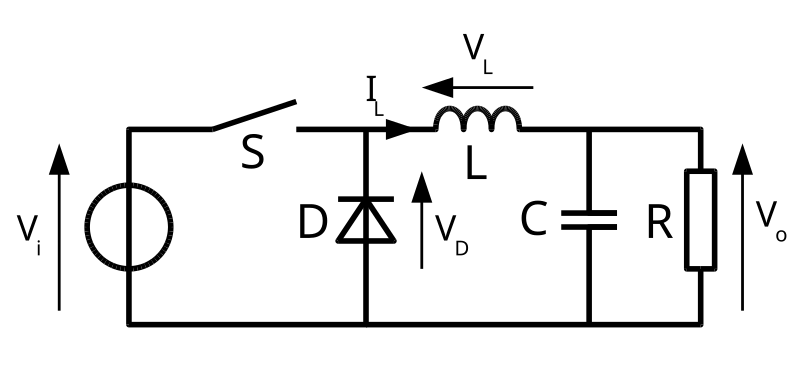
\includegraphics[width=\textwidth]{Imagenes/MPPT/Buck.jpg}
                        \caption{Componentes del Conversor Buck}
                        \label{fig:m1.1}
                    \end{subfigure}
                    \begin{subfigure}[b]{0.3\textwidth}
                        \centering
                        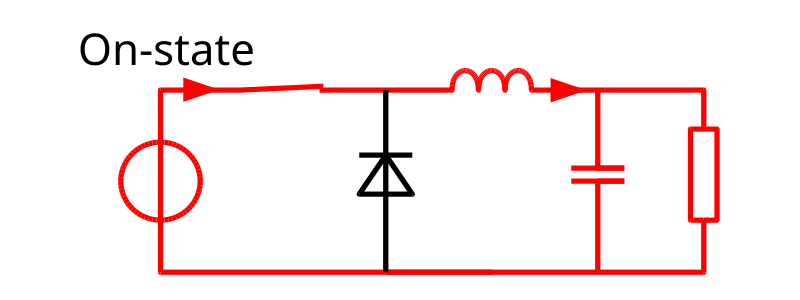
\includegraphics[width=\textwidth]{Imagenes/MPPT/Buck-On.jpg}
                        \caption{Estado On del Conversor Buck}
                        \label{fig:m1.2}
                    \end{subfigure}
                    \begin{subfigure}[b]{0.3\textwidth}
                        \centering
                        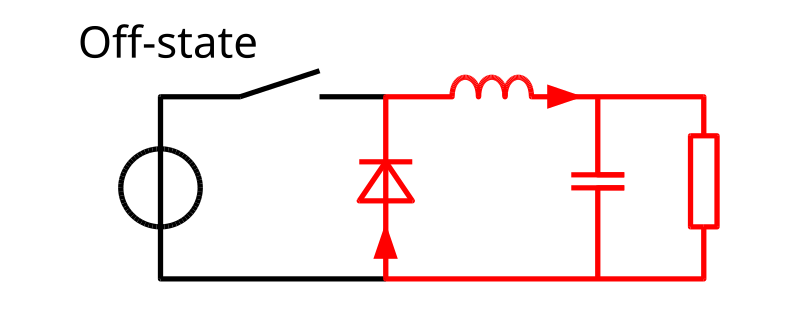
\includegraphics[width=\textwidth]{Imagenes/MPPT/Buck-Off.jpg}
                        \caption{Estado Off del conversor Buck.}
                        \label{fig:m1.3}
                    \end{subfigure}
                    \caption{Conversor Buck}
                    \label{fig:m1}
                \end{figure}

                Para entender este circuito, se debe hacer un análisis del estado transitorio del mismo en sus dos estados, On y Off. En principio, con el estado Off, la corriente en el circuito es nula. Cuando cambia al estado On, la corriente va empezar a subir y la bobina va a generar una caída de voltaje entre sus terminales. Esta caída de voltaje provoca que el voltaje resultante en la carga sea menor. A medida que pasa el tiempo, el índice de cambio de la corriente disminuye, y el voltaje en la bobina también disminuye, aumentando el voltaje en la carga. Durante este proceso, la bobina almacena energía en forma de campo magnético\par
                Cuando el interruptor de abre de vuelta (Off), la fuente de voltaje se remueve del circuito y la corriente disminuye. Esta corriente decreciente produce una caída de voltaje en la bobina (opuesto al generado en el estado On), y ahora la bobina se convierte en una fuente de corriente. La energía almacenada en el campo magnético de la bobina suporta el flujo de corriente por la carga. Esta corriente, que fluye mientras la fuente de voltaje está desconectada, cuando se suma a la corriente que fluye en el estado On, da como resultado una corriente de salida promedio mas grande que la que entrega la fuente de voltaje.\par

                \begin{figure} [!ht]
                    \centering
                    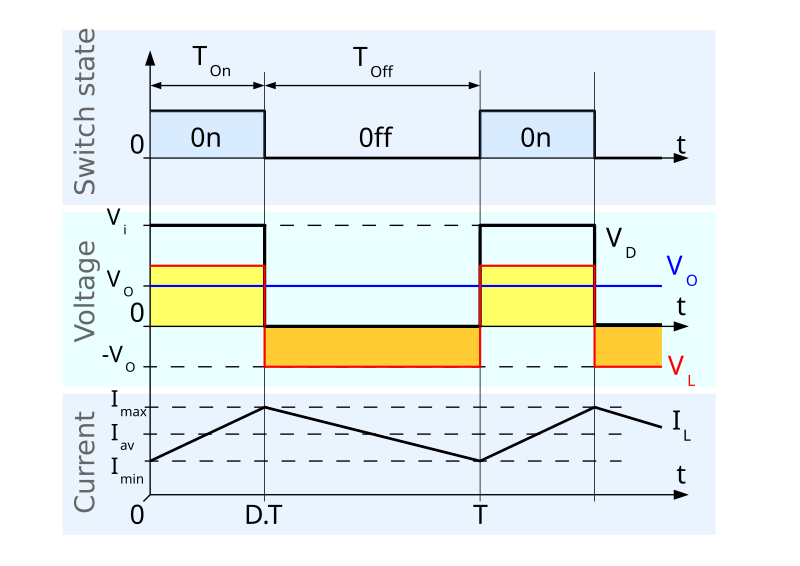
\includegraphics[width=0.6\linewidth]{Imagenes/MPPT/Gráfica.jpg}
                    \caption{Gráfica en el tiempo del comportamiento de las tensiones y corrientes de un convertidor buck.}
                    \label{fig:m1.4}
                \end{figure}
                
                Este aumento en la corriente promedio estaría compensando la reducción en el voltaje, manteniendo idealmente la potencia entregada en la carga. Si el switch se abre mientras la corriente sigue aumentando, entonces siempre va a haber una caída de tensión sobre la bobina, por lo tanto la carga siempre tendra menos voltaje que la entrada.\par

            \subsection{Sistema de Control}
                Si uno logra variar la frecuencia con la que ese switch se abre y se cierra, y al mismo tiempo medir la corriente y la tension recibida en la carga, se puede diseñar un sistema de control que, teniendo en cuenta esas variables, varíe esa frecuencia del interruptor con esas mediciones como realimentación, controlando una o la otra.\par
                El sistema de control que utilizamos es un control proporcional integral, o \textbf{PI}, siendo la aplicación de un control proporcional y uno integral al mismo tiempo.\par
                La parte proporcional de un control es el producto entre la señal de error ($e_{(t)}$) y la constante proporcional ($K_p$). Variando ($K_p$) se cambia la velocidad del control. Pero solo con un control proporcional se tiene error en régimen permanente, ya que este tipo de control requiere de error para entregar señal de control. La fórmula matemática que responde a esto es:\par
                \begin{equation}
                    P_{sal} = K_p \times e_{(t)}
                \end{equation}
                La parte integral del control actua cuando hay una desviación entre la variable y el punto de consigna, integrando esta desviación en el tiempo. El error es integrado, lo cual tiene la función de promediarlo o sumarlo por un período determinado, y luego se multiplica por una constante $K_i$. Elimina el error de estado estacionario, logrando seguimiento perfecto de la señal de referencia. La fórmula matemática que responde a esto es:\par
                \begin{equation}
                    I_{sal} = K_i \times \int e_{(t)} \ dt
                \end{equation}
                
        \section{Realización}
            \subsection{Esquemático}
                Se podrá encontrar el esquemático en el Apéndice A, que contiene los esquemáticos del proyecto.\par
            
            \subsection{Hardware}
                Para la realización de este cargador utilizamos una \textbf{RP2040 Zero}. Que luego se comunicará con el módulo de control para informar sobre los parámetros medidos.\par
                Para la medición de la corriente utilizamos un módulo \textbf{INA 219} que nos permite medir de forma precisa los parámetros de corriente.\par
                Para medir las tensiones tanto de entrada como de salida simplemente utilizamos divisores resistivos, los cuales nos devuelven voltajes proporcionales reducidos, tambien procesados por los otros dos ADCs de la RP2040 Zero. Para la conversion simplemente se tiene en cuenta la relacion de las resistencias.\par
                Para la alimentación del circuito se aprovecha el voltaje entregado por el cargador, donde conectamos una fuente stepdown que regula la tensión entregada por el cargador a 5V para la alimentación de la RP2040 Zero. Esto quiere decir que una vez que se conecta, el circuito ya se encuentra alimentado por energías renovables.\par
                En el circuito MPPT, la única diferencia con el teórico es el interruptor. Nuestro interruptor es un MOSFET canal P IRF4905, que resiste hasta 70A de corriente. Es necesaria la utilización de un MOSFET canal P porque la carga del mismo tiene que estar entre Drain y Masa, mientras que la carga de un canal N tiene que estar entre la alimentación y Source, algo que en nuestro diseño resultó inconveniente.\par
                Para conmutar este MOSFET con la RP2040, no solo fue necesaria la utilización de un transistor NPN, sino tambien la de un circuito totem pole\par
                Un circuito totem pole consta de 2 transistores, un PNP y un NPN, uno arriba del otro, con sus bases interconectadas. Esto nos permite conmutar el MOSFET sin problemas, porque admite corrientes en ambos sentidos, tanto positivas como negativas. Esto es necesario porque un MOSFET necesita ambos sentidos de corrientes. Para entrar en estado de corte, necesita una corriente positiva en el Gate, y para volver al estado de saturación, por las características capacitivas del mismo, genera una corriente negativa.\par
                Para el cálculo del inductor, se realizó el siguiente procedimiento:\par
                Fijándose en la figura \ref{fig:m1.4}, el aumento de la corriente en la bobina queda:\par
                \begin{equation}
                    \frac{di_L(t)}{dt} = \frac{V_L(t)}{L} = \frac{V_i - V_o}{L}
                \end{equation}
                y análogamente el descenso de la corriente es:\par
                \begin{equation}
                    \frac{di_L(t)}{dt} = \frac{V_L(t)}{L} = \frac{-V_o}{L}
                \end{equation}
                Como toda la energía que se almacena en la bobina durante el primer estado se transfiere durante el segundo, la energía del inductor al final del periodo de conmutación ($T_S$) es igual en $t = 0$ y en $t = T_S$.\par
                Por lo tanto, la tensión media en la bobina ⟨$V_L$⟩ en régimen permanente es nula, es decir, existe una igualdad en las áreas.\par
                \begin{equation}
                    \langle V_L \rangle = \frac{1}{T_S}\int_{T_S} V_L dt = 0
                \end{equation}
                Aplicando la ecuación se obtiene:\par
                \begin{equation}
                    (V_i - V_o) \cdot DT_S - V_o \cdot (T_S - DT_S) = 0
                \end{equation}
                Donde $D$ es un número adimensional, entre 0 y 1, denominado ciclo de trabajo. Siendo que este no puede ser mayor a 1, se cumple $V_o \leq V_i$, por tanto solo se podrá reducir la tensión.\par
                \begin{equation}
                    V_o = D \cdot V_i
                    \label{eq:D}
                \end{equation}
                La corriente media que circula por la bobina, con un D del 10\% (peor condición posible):\par
                \begin{equation}
                    I_L > \frac{I_{Lmax}}{10} = 1A
                \end{equation}
                
                \begin{equation}
                    \frac{\Delta I_L}{2} < 1A \Rightarrow \Delta I_L < 2A
                \end{equation}\\
                Para calcular la bobina, se utiliza la siguiente fórmula:\par
                \begin{equation}
                    \frac{V_i - V_o}{L} \cdot D \cdot T_S < 2A
                \end{equation}\\
                Reemplazando D por la equivalencia obtenida en la fórmula \ref{eq:D}, queda:\par
                \begin{equation}
                    L \geq \frac{V_o(1-\frac{V_o}{V_i})\cdot T_S}{2}
                \end{equation}
                Siendo\par
                    \[V_i [24V-48V]\]
                    \[V_o [24V-28V]\]
                    \[T_S = 32 \cdot 10^{-6} S  = 32KHz\]\\
                El máximo de esta función queda definido por los máximos valores de tensión de entrada y tensión de salida, por lo tanto:\par
                \begin{equation}
                    L \geq \frac{28 \cdot (1-\frac{28}{48}) \cdot 32 \cdot 10^{-6}}{2}
                \end{equation}
                Entonces \[L \geq 99,5\mu H\]\\
                La bobina utilizada en el circuito posee un valor de \textbf{$83 \mu H$}, la cual cumple con la condición anterior.\\
                Para el cálculo del capacitor correspondiente, se realizó el siguiente procedimiento:\\
                Cálculo para el ripple del capacitor de un 1\%:\par
                \begin{equation}
                    \Delta V_o = 1\% \cdot 28V = 0,28V
                \end{equation}
                La fórmula utilizada para obtener el valor del capacitor es la siguiente:\\
                \begin{equation}
                    \Delta V_o = \frac{V_o \cdot (1-\frac{V_o}{V_i})}{8 \cdot L \cdot C \cdot F^2}
                \end{equation}\\
                Despejando, se obtiene:\\
                \begin{equation}
                    C \geq \frac{V_o \cdot  (1 - \frac{V_o}{V_i})}{8 \cdot L \cdot \Delta V_o \cdot F^2}
                \end{equation}\\
                Con los valores ya calculados, se reemplazan los parámetros:\\
                \begin{equation}
                    C \geq \frac{28V \cdot (1 - \frac{28V}{36V})}{8 \cdot 83 \mu H \cdot 32KHz^2}
                \end{equation}
                Entonces \[C \geq 27,13 \mu F\]\\
                Para evitar resonancias, se estima que la frecuencia de resonancia tiene que estar 10 veces por debajo de la frecuencia en la que se trabaja. Por esto:\\
                \begin{equation}
                    \frac{F_S}{10} = \frac{1}{\sqrt{L \cdot C}}
                \end{equation}
                Despejando, queda:\\
                \begin{equation}
                    C = \frac{10^2}{32KHz^2 \cdot 27,13 \mu H} \simeq 2713 \mu F
                \end{equation}\\
                Por lo tanto, en el circuito final se utilizó un capacitor de \textbf{$3300 \mu F$}

            \subsection{Software}
                El sistema MPPT fue programado íntegramente con el lenguaje C sobre la RP2040.\par
                El microcontrolador lee las señales del divisor de tensión que caerá sobre sus ADC y, mediante una lógica dependiente de la relación entre las resistencias del divisor de tensión, el código interpreta estas señales para saber el valor deseado (ya sea corriente o votaje).\par
                Ya sabiendo los valores que se tienen que medir, se compararán con los valores definidos para el cambio de lógica. Así se define en que modo de carga estará el MPPT. Por ejemplo, para el cambio entre BULK y ABSORTION, el voltaje de la batería deberá ser mayor al voltaje máximo definido del modo BULK.\par
                Cada modo tiene su propia lógica para manejar el PWM que regula la tensión y corriente que le llega a la batería. En el modo BULK, primero se calcula el error entre la medicion actual y la deseada, luego se ve si la corriente que le llega a la batería es mayor o menor a la deseada y en base a esto se controla el PWM proporcionalmente e integralmente tomando en cuenta el error, pasando previamente por un saturador, asegurándose que el valor del PWM no sea ni mayor a 100\% ni menor a 0\%.\par
                Para conocer más sobre todo esto, referirse al Anexo B, más específicamente el Listing B.1.
                
            \section{Resultado Final}
                \begin{figure}[H]
                    \centering
                    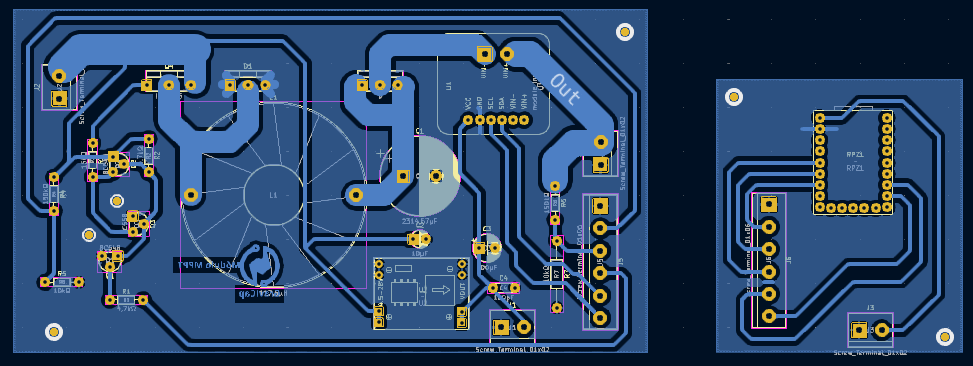
\includegraphics[width=0.8\linewidth]{Imagenes/MPPT/PCB - MPPT.jpg}
                    \caption{PCB del MPPT}
                    \label{fig:m5.1}
                \end{figure}

                \begin{figure}
                    \centering
                    \includegraphics[width=0.5\linewidth]{example-image}
                    \caption{PCB finalizado del MPPT}
                    \label{fig:m5.2}
                \end{figure}